% !TeX spellcheck = da_DK
\chapter{Activities og Intents}
\label{cha:activities-intents}

Indtil videre har vi kigget kort på vores MainActivity, som er entry point for en app. Hvis vi gerne vil have en ny activity, så skal vi starte denne med en intent. Dette kapitel vil kigge nærmere på en activity og dens livscyclus, forklare oprettelsen af nye activities, samt hvordan man kan starte disse activities med intents.

\section{Activities}

En activity er en komponent i en app, typisk er apps bygget op af flere aktiviteter, hvor hver activity har sin egen brugergrænseflade og layout, dermed kan en activity lidt sammenlignes med et vindue, man åbner på sin computer. Activities ligger som en stak i applikationen, hvilket betyder, at når man åbner en activity, svarer det til man åbner et nyt vindue, der ligger over det gamle, (og ofte skjuler det) og når den nye activity, lukkes kommer man så tilbage til den activity, man i sin tid åbnede den fra.

MainActivity er altid der vi starter. Når vi åbner en app, så det, der egentlig sker er, at vi starter vores MainActivity.


\subsection{Activity life cycle}

\begin{figure}[h]
	\begin{center}
		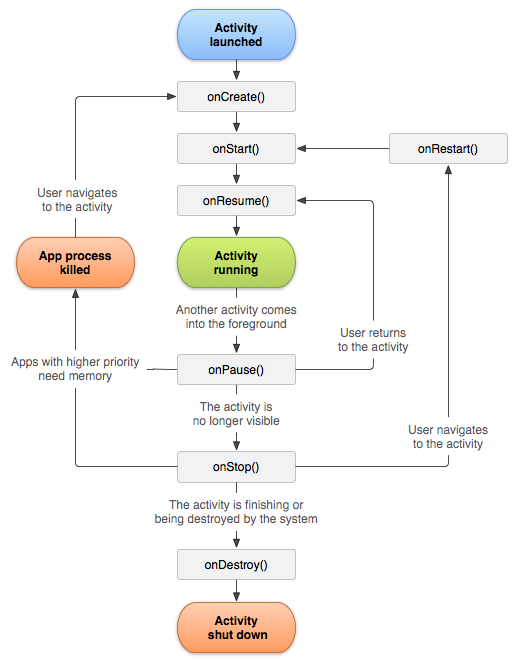
\includegraphics[width=7cm]{developerandroidcom_activitylifecycle.png}
		\caption{Activity lifecycle lånt af developer.android.com}
		\label{fig:android:activities:activitylifecycle}
	\end{center}
\end{figure}

I \autoref{fig:android:activities:activitylifecycle} vises de forskellige stadier, en activity er i, og kan hjælpe til at give et overblik over, hvornår de forskellige metoder bliver kaldt, og dermed også hvad man gerne vil have skal ske i de forskellige steps undervejs.

En activity vil typisk befinde sig i et af 4 stadier. Når activity'en er i forgrunden, og brugeren kan interagere med den, siger vi at den kører (running). Hvis en anden activity startes i forgrunden, men den gamle stadig er synlig siger vi at den er paused. Hvis en anden activity åbnes, så den gamle activity ikke længere kan ses, siger vi det er stopped. Paused og stopped activities kan lukkes af systemet for at frigøre hukommelse, i det tilfælde skal activity'en genstartes, når den skal bruges igen.

\subsection{Opsæt Views som objekter i Java}
Så skal vi endelig sætte layout og programmering sammen. Når I laver views så har hvert view et ID. Det er den I skal bruge når vi skal finde dem i Java. Det vi så gør er at erklære viewet som variabel og så får android til at finde den med \JavaInline|findViewByID|. Koden for at hente en knap ser ud som i \autoref{findviewbyid}

\begin{JavaCode}{Opsætte en knap i Java}{findviewbyid}
	Button button;
	
	@Override
	protected void onCreate(Bundle savedInstanceState) {
		super.onCreate(savedInstanceState);
		setContentView(R.layout.activity_main);
		
		button = (Button) findViewById(R.id.button);
	}
\end{JavaCode}

Ligesom alle objekter har knappen så nogle metoder som man bruger til at ændre eller få information om knappen. Der er eksempler på nogle af disse metoder i \autoref{buttonmethods}
\begin{JavaCode}{Metoder for button}{buttonmethods}
	button.setEnabled(false);
	//Deaktiver knappen saa den ikke kalder sin metode naar man trykker paa den
	
	button.setText("Klik mig");
	//Aendrer teksten paa knappen 
	
    button.setVisibility(View.INVISIBLE);
    //Goer knappen usynling. Den kan stadig trykkes paa
    
    button.setVisibility(View.VISIBLE);
    //Goer knappen synlig igen.
	
\end{JavaCode}
Der er mange flere metoder, og hver eneste view-element har sine specielle metoder. Vi kan på ingen måde liste dem alle sammen så søg på internettet efter elementernes metoder og hvad de gør. 


\subsection{Oprettelse af nye activities}

For at oprette en ny activity, starter vi med at lave en ny java fil ved siden af MainActivity.java (i ??? folderen) En ny activity skal altid nedarve fra Activity, ligesom MainActivity. 

\begin{JavaCode}{Eksempel på en activity.}{pop-up-activity}
	package com.example.housa.myapplication
	
	import android.app.Activity;
	import android.os.bundle;
	
	public class PopUpActivity extends Activity {
 
 @Override
 protected void onCreate(Bundle savedInstanceState) {
  super.onCreate(savedInstanceState);
  setContentView(R.layout.activity_popup);
 }
	}
\end{JavaCode}

Ud over at skrive selve Java koden, der definerer opførslen for en activity, skal den tilføjes til manifestet. Dette gøres ved at tilføje koden i \autoref{lst:add-activity-to-manifest} til manifestet inde i application tag'et.

\begin{XmlCode}{XML, der tilføjer PopUpActivity til manifestet.}{lst:add-activity-to-manifest}
	<activity android:name=".PopUpActivity" />
\end{XmlCode}

For at kunne starte ovenstående activity, skal vi benytte os af Intents, som vil blive forklaret i næste sektion.


\section{Intents}

En intent er en besked, man kan sende for at bede en anden komponent om at gøre noget. Intents kan bruges på flere forskellige måder, men de tre primære brugsscenarier er:

\subsubsection{Starte en anden activity}

Man kan starte en ny instans af en activity ved at sende en intent med som parameter til \JavaInline|startActivity()|. 

\subsubsection{Starte en service}

En service er en komponent, der kører i baggrunden og ikke har noget interface. Man starter en service på lidt samme måde som en activity, nemlig ved at sende en intent med som parameter til metoden \JavaInline|startService()|.

\subsubsection{Sende en broadcast}

En broadcast er en besked, som enhver app kan modtage. Der er forskellelige broadcasts for system events, som fx "foretag opkald" eller "opladning igang". Man kan sende en broadcast ved at sende en intent med som parameter til \JavaInline|sendBroadcast()| eller \JavaInline|sendOrderedBroadcast()|.
En standard broadcast kan ikke blive stoppet, og kan ikke videregive resultater. En orderedBroadcast vil sende broadcasten til alle relevante BroadCastRecievers en af gangen og tillade resultatet at propagere.

\subsubsection{Toasts}

En toast er en lill besked som popper op på skærmen de sættes ind ved hjælp af de her funktioner  

\begin{JavaCode}{Her kan man f.eks. vælge mellem en lang og en kort toast}{lst:toast-example}
	Toast toast = Toast.makeText(getActivity(), "Det her er min toast besked!", Toast.LENGTH_LONG.show(););
	toast.show();
	// Eller Toast.LENGTH_SHORT.show();
\end{JavaCode}

Som man kan se i \autoref{lst:toast-example} har toasteren brug for en activity, en besked og, hvor lang tid den skal vises.

\subsection{Explicit vs Implicit}

Der er to typer intents, explicitte og implicitte. I explicitte intents specificerer man præcist hvilken komponent, man vil have til at reagere. Da man kender navngivningen i ens egen app, vil dette være den typiske måde at håndtere kommunikationen indenfor ens egen app, som at starte nye activities inde i appen.

De implicitte intents fortæller ikke præcist hvilken komponent man vil have til at reagere, men i stedet hvilken handling man gerne ville have udført, så kan alle komponenter, der har den givne funktionalitet tilbyde at udføre handlingen. Dette benyttes fx, hvis man gerne vil have ens app til at sende en mail, men gerne bare vil bruge hvad end mailklient brugeren allerede har på telefonen.

\subsection{Start en activity med en Intent}

Først laves det intent vi vil starte vores activity med, her benyttes et explicit intent, da det skal benyttes til at starte en specifik activity i vores applikation. For at vores intent er explicit, skal vi definere hvilken klasse, den skal sendes til. For at starte den valgte activity, kalder vi derefter \JavaInline|startActivity|.

\begin{JavaCode}{Eksempel på et intent.}{explicit-intent}
	Intent intent = new Intent(this, PopUpActivity.class);
	startActivity(intent);
\end{JavaCode}

Man kan så afslutte en activity og gå tilbage til den forrige activity ved at kalde metoden \JavaInline|finish|. Man kan også lukke ens app helt ved at kalde \JavaInline|finish| i ens main activity.

Vi kan sende en besked med vores intent ved at benytte \JavaInline|putExtra| metoden, der tager en nøgle og en værdi som input.

\begin{JavaCode}{Sende en besked med et intent.}{putExtra-intent}
	public static final String POPUP_MESSAGE = "com.example.lukas.myapplication.POPUP_MESSAGE";
	...
	Intent intent = new Intent(this, PopUpActivity.class);
	intent.putExtra(POPUP_MESSAGE, "Hello World!");
	startActivity(intent);
\end{JavaCode}

\subsubsection{Adgang til meddelelsen fra et intent}

For at få fat i den besked vi sender med vha, \JavaInline|putExtra|, kan vi benytte \JavaInline|getIntent| fra den activity, der bliver startet med vores intent. Vi kan få fat i værdien i beskeden med \JavaInline|intent.get(Type)Extra(key)|, \todo{intent.get<<Type>>Extra(key)?} hvor ``\JavaInline|(Type)|'' skal udskiftes med typen på den værdi, man vil have fat i.

\begin{JavaCode}{Adgang til beskeden fra et intent.}{getExtra-intent}
	public class PopUpActivity extends Activity {
		
		@Override
		protected void onCreate(Bundle savedInstanceState) {
			super.onCreate(savedInstanceState);
			setContentView(R.layout.activity_popup);
			
			Intent intent = getIntent();
			String message = intent.getStringExtra(MainActivity.POPUP_MESSAGE);
			TextView textView = (TextView)findViewById(R.id.messageView);
			textView.setText(message);
			textView.invalidate();
		}
	}
\end{JavaCode}

\subsection{At få ting tilbage fra intents}
Hvad så hvis man vil have ting retur fra den activity man kalder? Du kan tilføje extras som ellers, men istedet for at kalde startActivity kalder du funktionen som i \autoref{forResultCall},
\begin{JavaCode}{Start en activity som giver et resultat}{forResultCall}
	startActivityForResult(intent, REQUEST_CODE);
\end{JavaCode}
Hvor request koden er en integer. Den bruger vi senere så husk den. Vi laver så en metode til at modtage resultatet i den activity vi kalder startActivityForResult i. Denne metode ser ud som i \autoref{onActivityResult}
\begin{JavaCode}{Få resultatet}{onActivityResult}
	protected void onActivityResult(int requestCode, int resultCode, Intent intent){
		//Soerg for at requestcode er lig den request code du sendte
		//og at resultcode er lig Activity.RESULT_OK
		//Det resultat du faar ligger i intentet som extra
		//Her er et eksempel med en string
		intent.getStringExtra("resultat");
	}
\end{JavaCode}

Og hvordan skal det så se ud i den activity du kalder? Her skal det se ud som i \autoref{resultatTilbage}.
\begin{JavaCode}{Send et resultat tilbage}{resultatTilbage}
	Intent intentresult = new Intent();
	intent.putExtra("resultat", resultat);
	setResult(REQUEST_CODE, intent)
	finish();
\end{JavaCode}
Request code er til hvis en aktivitet skal modtage fra eller returnere til flere andre activities. Så kan man kende forskel på dem med request code. 

\subsection{Start en activity fra en anden app med en Intent}

Vi kan inkorporere aktiviteter fra andre apps, hvis de lytter efter intents. Et eksempel er en e-mail-app, vi kan bruge den indbyggede e-mail-klient (eller en anden e-mail-klient) til at sende en email fra vores app. Vi skal bruge implicitte intents til dette formål, da vi ikke nødvendigvis kender klassen samt stien til e-mail-klientens aktivitet, og vi vil muligvis gerne have brugeren til at vælge den e-mail-app, som de bedst kan lide.

For at skabe sådan en implicit intent, skaber vi simpelthen en ny intent, sætter den relevante handling, og giver den de nødvendige metadata, så aktiviteten, der modtager intent'en, kan fuldføre opgaven.

Vi vil genbruge e-mail-eksemplet. Hvis vi ønsker at sende en email fra vores app, bruger vi handlingen \JavaInline|Intent.ACTION_SEND|. Handlingen \JavaInline|ACTION_SEND| betyder, at vi vil sende nogle data.

\begin{JavaCode}{Eksempel på et implicit intent.}{lst:implicit-intent}
	Intent mailIntent = new Intent();
	mailIntent.setAction(Intent.ACTION_SEND);
\end{JavaCode}

Nu når vi har en intent med den relevante handling, skal vi indstille metadataene for vores intent således, at den modtagende aktivitet ved, hvad den skal gøre med intent'en. Hvis du sender en mail, skal du sætte typen af intent'en til ``text/html'' og e-mail-adresse, emne og indhold til e-mailen tilføjes som vist i \autoref{lst:mailsending-intent}:

\begin{JavaCode}{Eksempel på et mail sendende intent.}{lst:mailsending-intent}
	public void sendMail(View view) {
		Intent mailIntent = new Intent();
		mailIntent.setAction(Intent.ACTION_SEND);
		mailIntent.setType("text/html");
		mailIntent.putExtra(Intent.EXTRA_EMAIL, "test@someone.com");
		mailIntent.putExtra(Intent.EXTRA_SUBJECT, "NEWS");
		mailIntent.putExtra(Intent.EXTRA_TEXT, "Some mail content");
		startActivity(Intent.createChooser(mailIntent, "Send Mail"));
	}
\end{JavaCode}

\subsection{Start en activity med en Intent fra en anden app}

For at modtage en implicit intent, skal du oprette den activity, der skal modtage intent'en, for eksempel kan det være en activity, der fanger ``send'' intent'en, men i stedet for at sende den, viser den faktisk mailen.

Først skal du oprette activity'en. Bare lav en tom aktivitet som i \autoref{lst:empty-activity}.

\begin{JavaCode}{Tom activity}{lst:empty-activity}
	public class FakeMailActivity extends Activity {
		@Override
		protected void onCreate(Bundle savedInstanceState) {
			super.onCreate(savedInstanceState);
		}
	}
\end{JavaCode}

Tilføj nu den nye activity til manifestet og giv den et filter, der fanger intents sendt fra ``text/html'' mimeTypes.

\begin{XmlCode}{XML, der tilføjer FakeMailActivity til manifestet.}{lst:add-activity-with-filter-to-manifest}
	<activity android:name=".FakeMailActivity">
		<intent-filter>
			<action android:name="android.intent.action.SEND" />
			<category android:name="android.intent.category.DEFAULT"/>
			<data android:mimeType="text/html" />
		</intent-filter>
	</activity>
\end{XmlCode}

Nu, når du sender ``Send'' intent'en for ``text/html'', vil den spørge, om du vil bruge Mail-appen eller vores egen app.

\begin{figure}[h]
	\begin{center}
		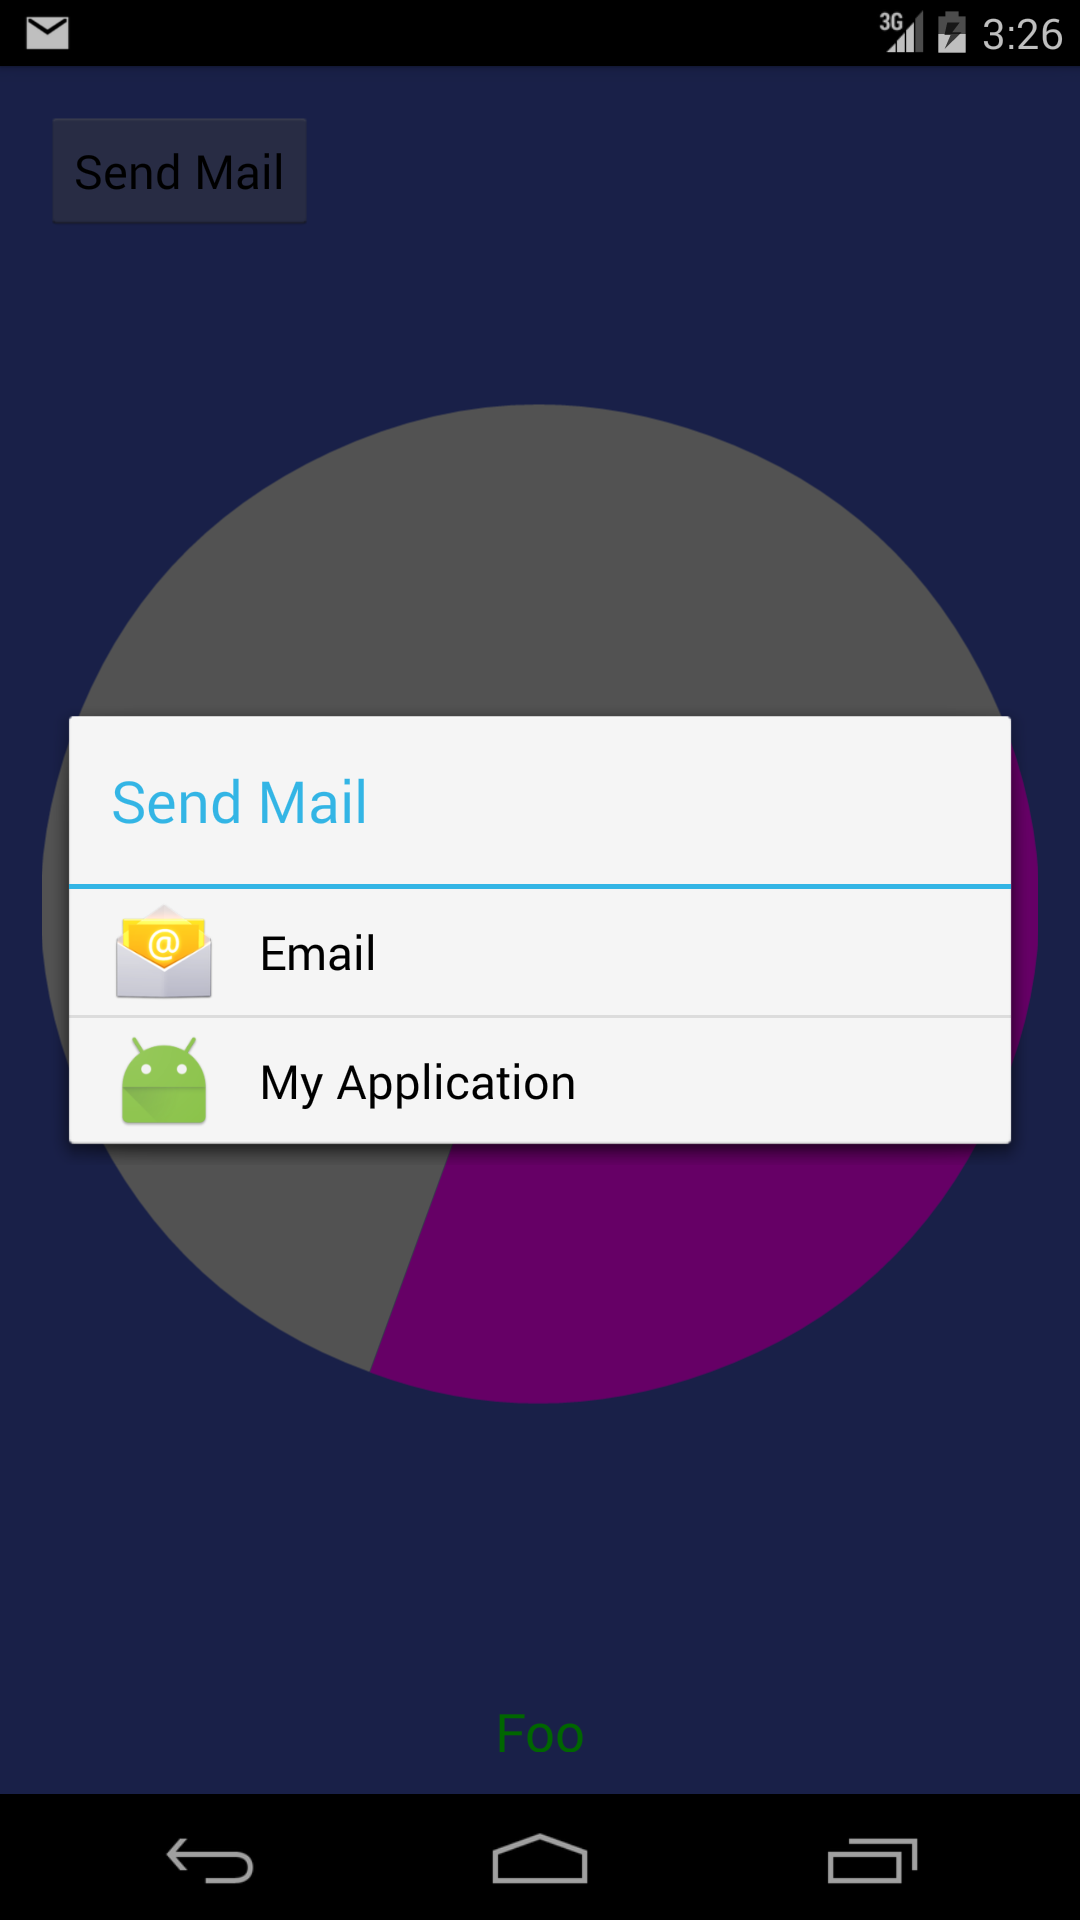
\includegraphics[width=7cm]{email_chooser.png}
		\caption{Email vælger}
		\label{fig:android:activities:email_chooser}
	\end{center}
\end{figure}

\subsubsection{BroadcastReceivers}

Din app kan sende en intent som en broadcast, og Android-systemet sender hele tiden broadcasts. For at modtage en sådan broadcast, har du brug for en \JavaInline|BroadcastReceiver|-klasse, som kan se ud som \autoref{lst:broadcast-receiver}.

\begin{JavaCode}{BroadcastReciever}{lst:broadcast-receiver}
	public class NoPhoneCallsReceiver extends BroadcastReceiver {
		@Override
		public void onReceive(Context context, Intent intent) {
		}
	}
\end{JavaCode}

Vi kunne få denne broadcastreceiver til, at modtage broadcasten ``OutgoingCalls'', vi skal blot tilføje den til manifestet (på samme sted, hvor du ville tilføje en ny aktivitet) og give det et intentfilter som i \autoref{lst:add-broadcastreceiver-to-manifest}.

\begin{XmlCode}{BroadcastReceiver til opkald}{lst:add-broadcastreceiver-to-manifest}
	<receiver android:name=".NoPhoneCallsReceiver">
		<intent-filter>
			<action android:name="android.intent.action.NEW_OUTGOING_CALL" />
		</intent-filter>
	</receiver>
\end{XmlCode}

Opsnapning af disse udgående telefonopkald, broadcasts, kan have mange anvendelser, såsom at ringe dine venner op via VoIP i stedet for via telefonnetværket, eller man kan sørge for, at den korrekte områdekode er vedhæftet, eller for at blokere alle opkald til numre, der ikke er på en forældrekontrol whitelist.

En sjov ting at gøre, kunne også være at få denne broadcastreciever til at stoppe alle udgående telefonsamtaler, som i \autoref{lst:no-calls-receiver}.

\begin{JavaCode}{At stoppe udgående opkald.}{lst:no-calls-receiver}
	public class NoPhoneCallsReceiver extends BroadcastReceiver {
		@Override
		public void onReceive(Context context, Intent intent) {
			setResultData(null);
		}
	}
\end{JavaCode}

\begin{exercise}
	Lav en app, der har en main activity og en anden activity, der viser et billede. Tilføj en knap til din main activity, der åbner din anden activity.
\end{exercise}

\begin{exercise}
	Lav en app, der har en main activity og en anden activity med et EditText felt. Tilføj en knap og et \JavaInline|EditText|felt til din main activity, der åbner din anden activity og viser teksten fra \JavaInline|EditText| i din main activity.
\end{exercise}

\begin{exercise}
	Lav en Activity, der har en ‘send Email’ knap, der åbner en Email dialog
\end{exercise}

\begin{exercise}
	Lav en activity, der agerer som et alternativ til email klienten, når man trykker på ‘send mail’ knappen fra opgave 3
\end{exercise}

\begin{exercise}
	Lav en \JavaInline|BroadCastReciever|, der blokerer alle udgående opkald.
\end{exercise}

\begin{exercise}
	Lav en activity, der sender en \JavaInline|Broadcast|, og en \JavaInline|BroadCastReciever|, der modtager den givne \JavaInline|BroadCast|.
\end{exercise}

